% Тут используется класс, установленный на сервере Papeeria. На случай, если
% текст понадобится редактировать где-то в другом месте, рядом лежит файл matmex-diploma-custom.cls
% который в момент своего создания был идентичен классу, установленному на сервере.
% Для того, чтобы им воспользоваться, замените matmex-diploma на matmex-diploma-custom
% Если вы работаете исключительно в Papeeria то мы настоятельно рекомендуем пользоваться
% классом matmex-diploma, поскольку он будет автоматически обновляться по мере внесения корректив
%

% По умолчанию используется шрифт 14 размера. Если нужен 12-й шрифт, уберите опцию [14pt]
%\documentclass[14pt]{matmex-diploma}
\documentclass[14pt]{matmex-diploma-custom}
\usepackage{graphicx}
\usepackage{multirow}
\usepackage{fancyvrb}
\usepackage[misc,geometry]{ifsym} 
\usepackage{subcaption}

\usepackage{tikz}

\begin{document}
\usetikzlibrary{calc}
\usetikzlibrary{shapes,arrows}
\usetikzlibrary{arrows,automata}
\usetikzlibrary{positioning}
\newcommand{\tikzmark}[1]{\tikz[overlay,remember picture] \node (#1) {};}
\def\Put(#1,#2)#3{\leavevmode\makebox(0,0){\put(#1,#2){#3}}}

\newcommand{\ltz}{$< 1$}
\tikzset{
    state/.style={
           rectangle,
           rounded corners,
           draw=black, very thick,
           minimum height=2em,
           inner sep=2pt,
           text centered,
           },
}
\def\figurename{Рис}

% Год, город, название университета и факультета предопределены,
% но можно и поменять.
% Если англоязычная титульная страница не нужна, то ее можно просто удалить.
\filltitle{ru}{
    chair              = {Программная инженерия},
    title              = {Комбинирование нейронных сетей и синтаксического анализа для предсказания вторичных структур генетических цепочек},
    % Здесь указывается тип работы. Возможные значения:
    %   coursework - Курсовая работа
    %   diploma - Диплом специалиста
    %   master - Диплом магистра
    %   bachelor - Диплом бакалавра
    type               = {coursework},
    position           = {студента},
    group              = 571,
    author             = {Лунина Полина Сергеевна},
    supervisorPosition = {к.\,ф.-м.\,н., доцент},
    supervisor         = {Григорьев С.\,В.},
    %reviewerPosition   = {Специалист по анализу данных ООО "Интеллоджик"},
    %reviewer           = {Малыгина Т.\,С.},
    chairHeadPosition  = {д.\,ф.-м.\,н., профессор},
    chairHead          = {Терехов А.\,Н.},
%   university         = {Санкт-Петербургский Государственный Университет},
%   faculty            = {Математико-механический факультет},
%   city               = {Санкт-Петербург},
%   year               = {2020}
}
\filltitle{en}{
    type               = {coursework},
    chair              = {Software Engineering},
    title              = {The composition of neural networks and parsing for genomic sequences secondary structure prediction},
    author             = {Polina Lunina},
    supervisorPosition = {Assistant Professor},
    supervisor         = {Semyon Grigorev},
  %  reviewerPosition   = {Data scientist at Intellogic LLC},
  %  reviewer           = {Tatiana Malygina},
    chairHeadPosition  = {Professor},
    chairHead          = {Andrey Terekhov},
}
\maketitle
\tableofcontents
% У введения нет номера главы
\section*{Введение}
В биоинформатике существует множество задач анализа генетических цепочек, например, классификация организмов по их генетическим данным, поиск подпоследовательностей и другие. Для решения этих задач требуется разработка новых алгоритмов и совершенствование существующих, и при этом в основе различных методов анализа биологических данных лежат некоторые общие базовые принципы.

Молекула РНК представляет собой цепочку нуклеотидов (первичная структура), и в том случае, когда два фрагмента этой цепи соединяются друг с другом, перегибаясь и образуя на конце неспаренный участок --- петлю, формируется элемент, называемый в
биологии стемом. И совокупность стемов различных размеров, а также вложенных стемов составляет сложную и стабильную вторичную структуру. Известно, что вторичная структура содержит в себе важную для идентификации организма информацию, поэтому среди алгоритмов для решения различных задач анализа цепочек РНК наибольшим успехом пользуются те, что ее каким-либо образом учитывают. Существуют различные методы формального описания вторичной структуры, например, скрытые марковские модели, ковариационные модели~\cite{EddyDurbin} и формальные грамматики~\cite{LWPCFG,PCFG,GrammarsRNA}.

При работе с биологическими данными важно учитывать присутствие в них шумов и мутаций, что делает точные алгоритмы неприменимыми и требует проведения некоторой вероятностной оценки. Популярным способом обработки зашумленных данных являются методы машинного обучения, в частности, нейронные сети, которые в настоящее время успешно используются в биоинформатике~\cite{ANN,Humidor}.

В рамках предыдущей дипломной работы был предложен новый подход для решения задач обработки последовательностей, обладающих некоторой синтаксической структурой. Данный подход основан на комбинировании методов синтаксического анализа и машинного обучения. Предлагается использовать грамматику для кодирования характерных особенностей синтаксической структуры, алгоритм синтаксического анализа --- для их поиска во входных данных, а обработку информации о наличии и расположении этих особенностей в цепочке и вероятностную оценку провести с помощью нейронной сети, сконструированной для решения конкретной задачи. И, применительно к генетическим данным, синтаксической структурой является вторичная структура РНК, а искомыми особенностями --- составляющие ее стемы. 

Направлением исследования, представленного в данной работе, является предсказание вторичных структур РНК с использованием разработанного в предыдущей работе подхода. Синтаксический анализатор находит во входной строке все подстроки, которые удовлетворяют правилам образования стемов, описанным в грамматике. Однако такое множество подстрок описывает все теоретически возможные в заданной последовательности стемы, закодированные средствами используемой грамматики, а реальная вторичная структура РНК живого организма содержит только небольшое их подмножество. Кроме того, существуют более сложные особенности вторичной структуры, невыразимые простой контекстно-свободной грамматикой, такие как псевдоузлы и неклассические пары комплиментарности оснований. Поэтому для генерации чистой вторичной структуры из результата работы парсера в рамках предложенного подхода предлагается использовать нейронную сеть, задача которой в данном случае --- отфильтровать лишние стемы и достроить невыразимые в грамматике элементы.

\section{Постановка задачи}
Целью данной работы является исследование возможности применения предложенного в предыдущей дипломной работе подхода к задаче предсказания вторичных структур геномных последовательностей. Для реализации данной цели были поставлены следующие задачи.
\begin{itemize}
    \item Разработка общей архитектуры решения.
    \item Проведение экспериментальных исследований.
    \begin{itemize}
        \item Предсказание вторичных структур транспортных РНК фиксированной длины.
        \item Предсказание вторичных структур транспортных РНК произвольной длины.
        \item Исследование возможности предсказания псевдоузлов, невыразимых средствами используемой грамматики.
    \end{itemize}
\end{itemize}

\section{Обзор используемого подхода}
Предложенный в предыдущей дипломной работе подход для анализа вторичной структуры последовательностей основан на комбинировании нейронных сетей и синтаксического анализа. Основная идея заключается в том, что характерные элементы вторичной структуры последовательностей необходимо формально описать средствами простой (контекстно-свободной) грамматики, а затем для поиска в некоторой строке подстрок, подходящих под это описание (формально --- выводимых из стартового нетерминала грамматики), использовать матричный алгоритм синтаксического анализа. Результат работы такого алгоритма --- матрица разбора --- будет хранить информацию о выводимости всех подстрок данной строки в используемой грамматике, что с практической точки зрения означает наличие и взаимное расположение искомых характерных элементов. Завершающим этапом в рамках предложенного подхода является обработка матриц разбора, преобразованных в некоторый удобный формат, с помощью искусcтвенных нейронных сетей для решения конкретной поставленной задачи (например, классификация генетических цепочек). 

Опишем более формально описанные выше концепции применительно к задачам в области биоинформатики, где рассматриваемыми последовательностями являются цепочки РНК различных организмов, а кодируемым в грамматике элементом является стем вторичной структуры. Первичная структура молекулы РНК представляет собой последовательность нуклеотидов, т.е. символов алфавита \{A, C, G, U\}. Некоторые участки такой последовательности могут соединяться между собой, образуя характерные элементы --- стемы, состоящие из спаренного участка (стебля) и неспаренного (петли), как показано на рис.~\ref{molekula}. Вторичная структура молекулы РНК состоит из комбинации стемов различного размера и степени вложенности, и общий вид таких конструкций необходимо формализовать в грамматике.

\begin{figure}[h]
\begin{center}
\centering
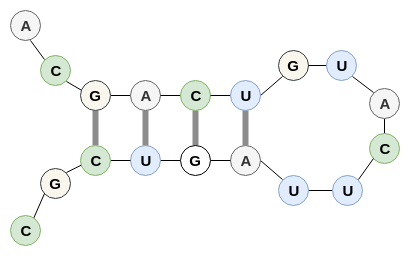
\includegraphics[width=5.8cm]{pics/molekula.png}
\caption{Образование вторичной структуры молекулы РНК}
\label{molekula}
\end{center}
\end{figure} 

\subsection{Грамматика}
В данной работе для описания стемов вторичной структуры была использована контекстно-свободная грамматика $G_0$ (рис.~\ref{gram}), предложенная в предыдущей работе. Эта грамматика учитывает классические правила формирования нуклеотидных пар $A-U$, $C-G$ (строка \textbf{5}) и описывает рекурсивные композиции стемов высоты от трех и более (строки \textbf{7-12}). Размер петли внутри стема лежит в пределах от двух до десяти нуклеотидов, такую же длину имеют последовательности, расположенные между любыми двумя стемами (строка \textbf{2}). Эти числа были получены путем экспериментов и теоретических исследований реальных вторичных структур РНК и могут быть изменены в рамках решения конкретной задачи.

\begin{figure}[h]
\begin{Verbatim}[numbers=left,xleftmargin=5mm]
s1: stem<s0>
any_str : any_smb*[2..10]
s0: any_str | any_str stem<s0> s0
any_smb: A | U | C | G
stem1<s>: A s U | G s C | U s A | C s G 
stem2<s>: stem1< stem1<s> >
stem<s>:  
      A stem<s> U 
    | U stem<s> A 
    | C stem<s> G 
    | G stem<s> C 
    | stem1< stem2<s> >  
\end{Verbatim}
\caption{Контекстно-свободная грамматика $G_0$ для описания стемов вторичной структуры РНК}
\label{gram}
\end{figure}

\subsection{Синтаксический анализатор}
Синтаксический анализ в данном случае используется для поиска всех подстрок некоторой строки, выводимых из стартового нетерминала грамматики $G_0$, т.е. тех участков этой строки, которые в терминах $G_0$ являются стемами вторичной структуры. Формально, для входной строки $w$ парсер сформирует верхнетреугольную булеву матрицу разбора $M$, где $M[i,j]=1$, тогда и только тогда, когда подстрока $w[i,j]$  выводима из стартового нетерминала грамматики. 

В данной работе был использован разработанный в рамках проекта YaccConstructor~\cite{yacc} в лаборатории JetBrains~\cite{jetbrains} алгоритм, основанный на матричных операциях~\cite{Azimov:2018:CPQ:3210259.3210264}, который демонстрирует высокую производительность на практике в связи с использованием параллельных вычислений.

\subsection{Искусственные нейронные сети}
Для анализа данных, проведения вероятностной оценки и генерации конечного результата в рамках некоторой задачи далее используются нейронные сети. Входными данными здесь являются матрицы, полученные парсером (при необходимости подвергнутые некоторой пост-обработке и приведенные в удобный формат), а выходные данные зависят от особенностей конкретного исследования, например, класс, к которому принадлежит каждая цепочка для проблемы классификации организмов. Архитектура сетей, их количество и шаги, предпринятые для промежуточной обработки всех данных, также зависят от специфики поставленной задачи.

\section{Архитектура решения}
\subsection{Формальное представление вторичной структуры молекулы РНК}
Вторичная структура молекулы РНК представляет собой комбинацию вложенных стемов различной высоты и размера петли. Пример вторичной структуры транспортной РНК (тРНК) представлен на рис.~\ref{struc_a}. Формально такой объект можно представить разными способами, но самыми популярными являются следующие два.
\begin{itemize}
    \item Матрица контактов, описывающая наличие или отсутствие связи между каждыми двумя нуклеотидами --- верхнетреугольная матрица $M$, где $M[i,j]=1$ тогда и только тогда, когда между символами цепочки в позициях $i$ и $j$ существует контакт во вторичной структуре.
    \item Строка в формате dot-bracket, где каждому символу цепочки сопоставлен один из символов алфавита \{.()\{\}<>\}. Здесь точка обозначает неспаренный нуклеотид, открытая скобка указывает на то, что нуклеотид сопряжен с некоторым другим впереди него, а закрытая --- на то, что нуклеотид сопряжен с некоторым другим позади него. Другие виды скобок предназначены для представления более сложных элементов, в частности, псевдоузлов.
\end{itemize}

Такие форматы описания вторичных структур повсеместно используются как в базах данных вторичных структур живых организмов, так и в различных инструментов для их предсказания.

\subsection{Задача предсказания вторичной структуры РНК в рамках предложенного подхода}
В данном разделе рассмотрим общую мотивацию применения подхода, основанного на комбинации методов синтаксического анализа и машинного обучения, к задаче предсказания вторичных структур РНК различных организмов. 

Синтаксический анализатор находит все теоретически возможные в правилах заданной грамматики стемы, однако реальная вторичная структура содержит далеко не все из них, так как грамматикой мы описали только общий вид стема, но не учли особенности их взаимного расположения и различные термодинамические и биологические законы, которые тяжело поддаются формализации. Поэтому для использования предложенного подхода в рамках задачи генерации чистой вторичной структуры живого организма необходимо обработать полученные матрицы разбора и отфильтровать лишние стемы и, возможно, достроить те элементы вторичной структуры, которые невыразимы средствами данной грамматики. Например, важным элементом вторичной структуры РНК являются так называемые псевдоузлы, которые состоят из двух шпилек, где половина стебля одной шпильки располагается между двумя половинами стебля другой шпильки. Однако псевдоузлы невыразимы средствами контекстно-свободных грамматик. Кроме того, в реальных вторичных структурах иногда встречаются неклассические пары нуклеотидов (например, $U-G$), но включение их в грамматику приведет к кратному увеличению количества правил и, как следствие, к существенным затратам по времени на синтаксический анализ.

Таким образом, для преобразования результата работы парсера в корректную вторичную структуру предлагается использовать нейронную сеть, для которой входным слоем будет матрица разбора в некотором формате, а выходным --- сгенерированная по ней вторичная структура.

Как было описано в разделе 2.2, результат работы парсера на входной строке --- верхнетреугольная булева матрица, где единица в позиции $[i,j]$ означает тот факт, что подстрока этой строки от $i$ до $j$ свернется в стем по правилам грамматики. В то же время, в разделе 3.1 было рассмотрено матричное представление вторичной структуры, в котором единица в позиции $[i,j]$ указывает на наличие контакта между нуклеотидами $i$ и $j$. Несложно заметить, что данные обозначения эквиваленты, поэтому, обрабатывая матрицы разбора, мы имеем дело с данными в классическом формате представления вторичной структуры. Примеры таких матриц для реальной вторичной структуры тРНК продемонстрированы на рис.~\ref{struc}.

Удобным форматом данных для обучения нейронной сети являются изображения, поэтому мы предлагаем привести матрицу разбора и матрицу контактов к черно-белым изображениям следующим образом: единицы заменить на белые пиксели, а нули на черные. И такие изображения использовать для обучения и тестирования нейронных сетей.

\begin{figure}[h]
\centering
\begin{subfigure}{.3\textwidth}
  \centering
  \fbox{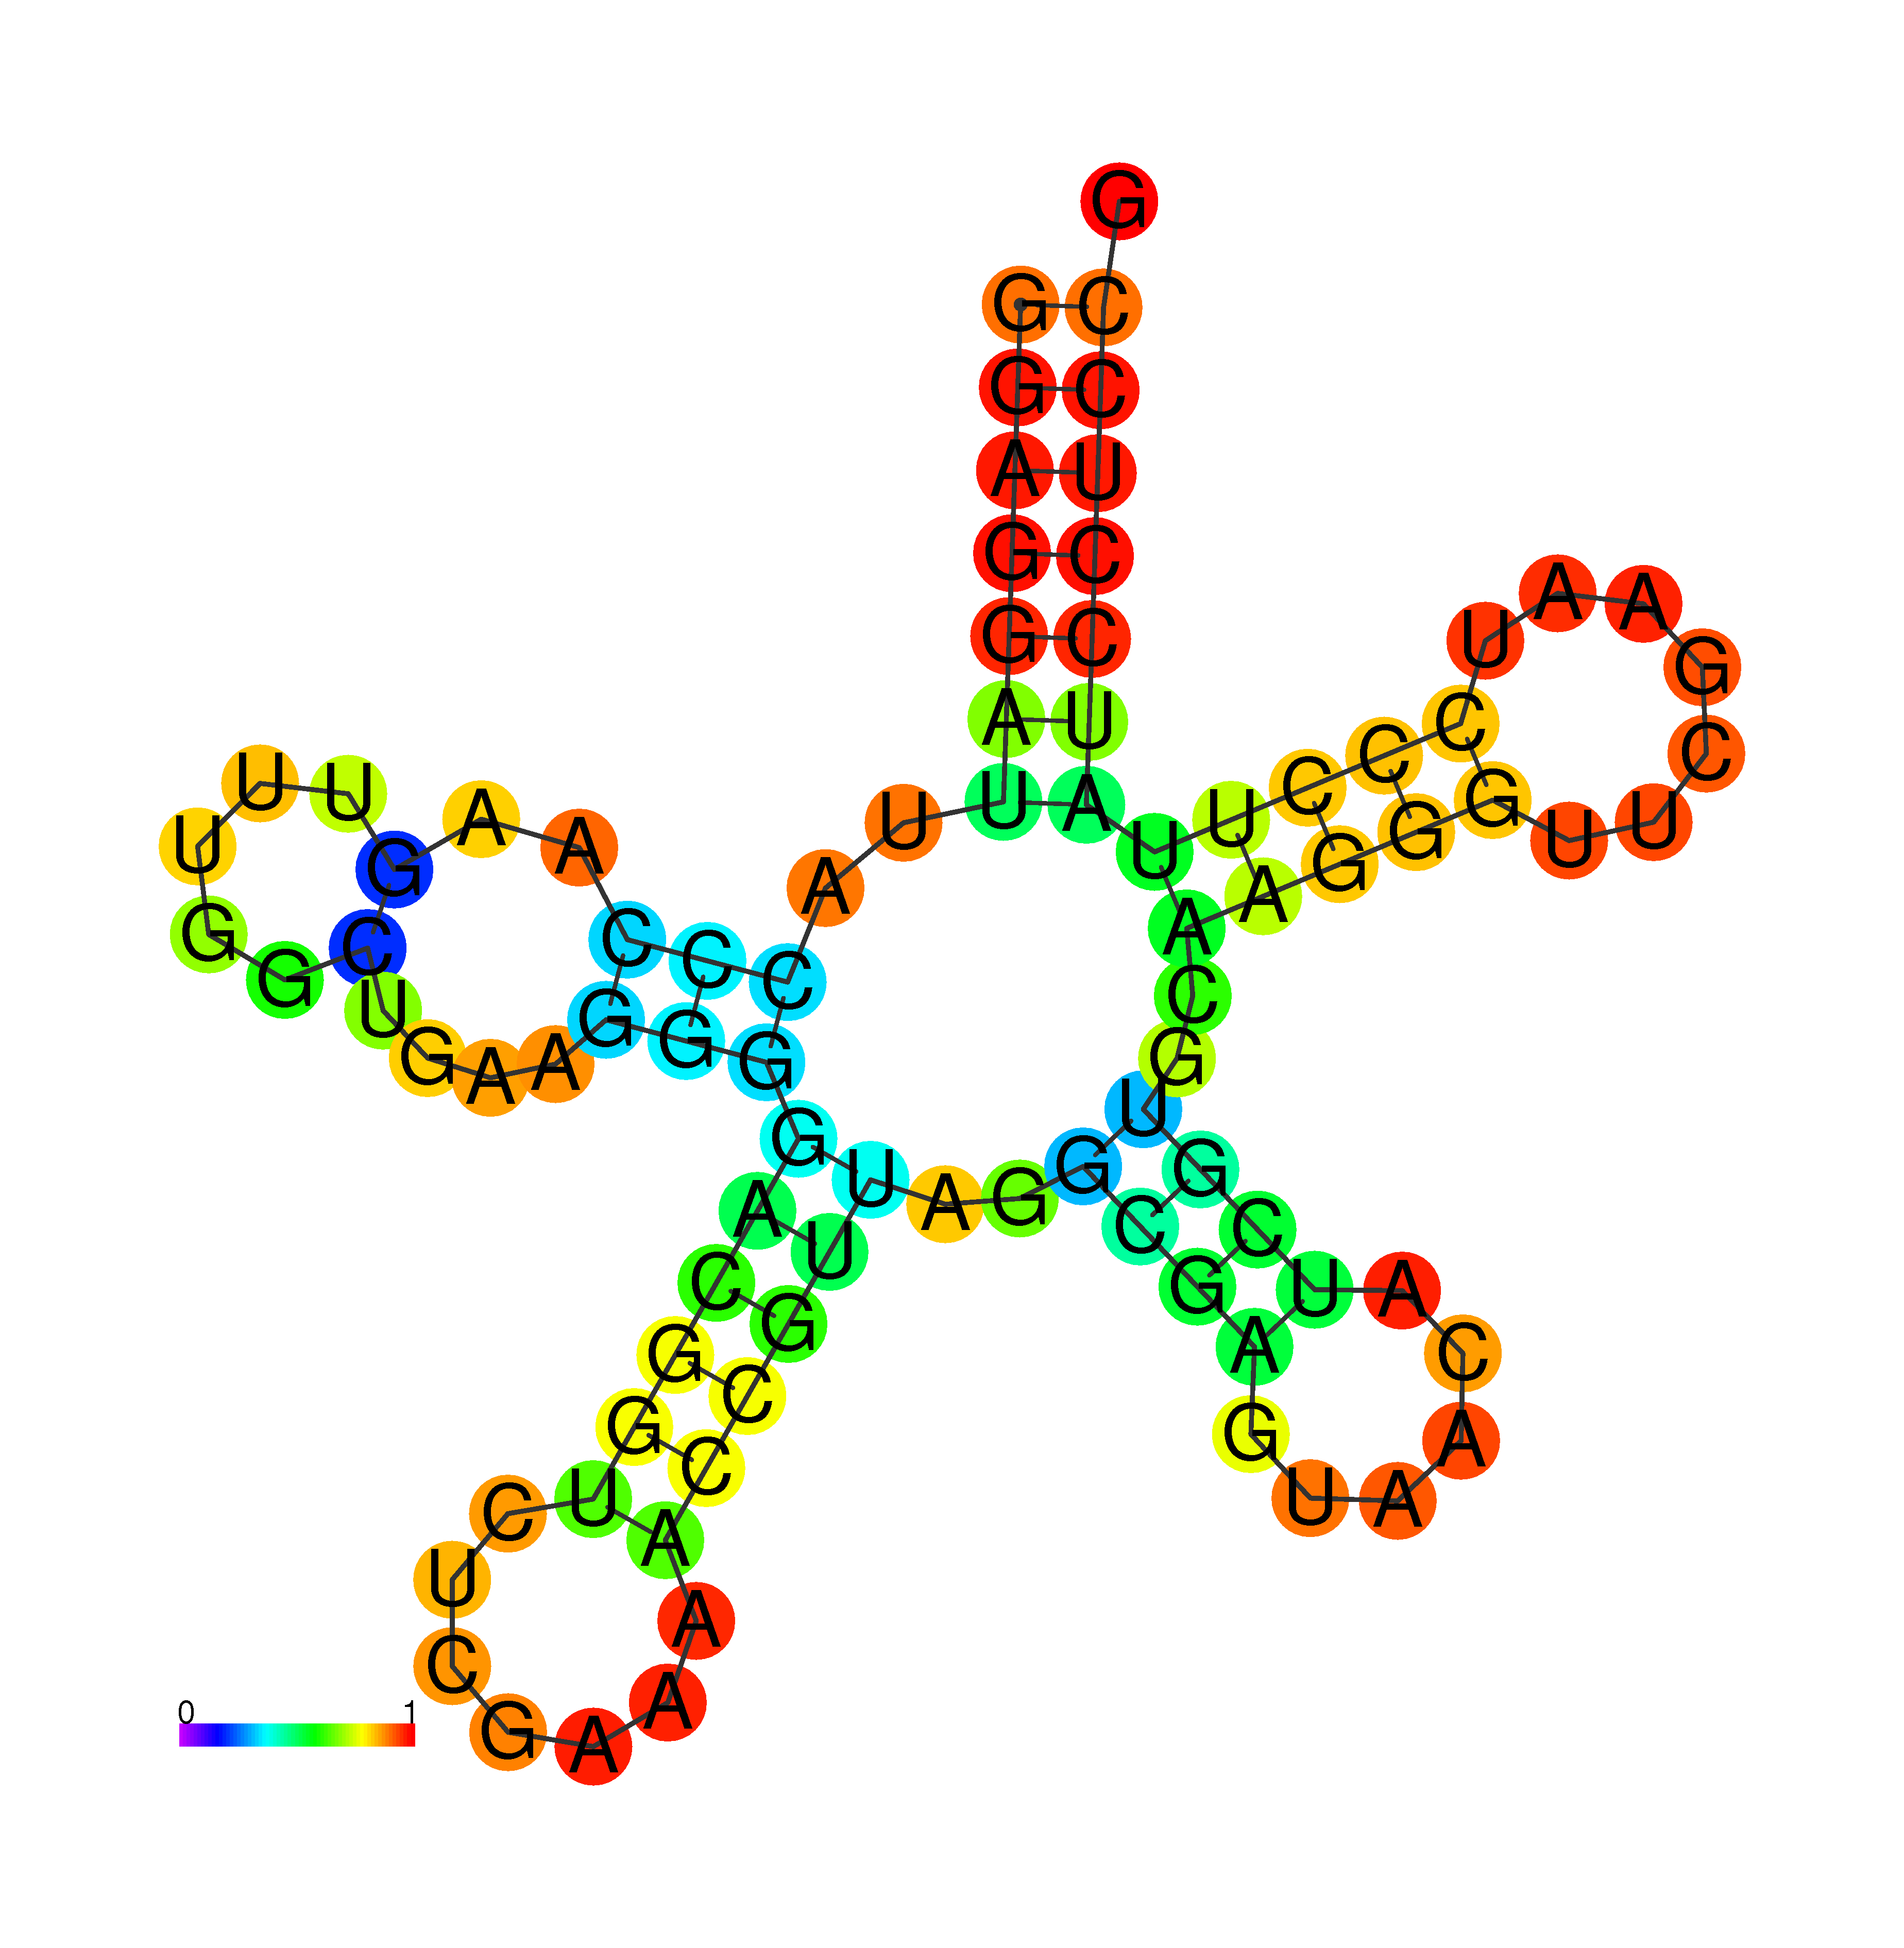
\includegraphics[width=.8\linewidth]{pics/structure.png}}
  \caption{Вторичная структура}
  \label{struc_a}
\end{subfigure}%
\begin{subfigure}{.3\textwidth}
  \centering
  \fbox{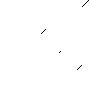
\includegraphics[width=.8\linewidth]{pics/etalon.png}}
  \caption{Матрица контактов}
  \label{struc_b}
\end{subfigure}
\begin{subfigure}{.3\textwidth}
  \centering
  \fbox{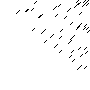
\includegraphics[width=.8\linewidth]{pics/parsed.png}}
  \caption{Матрица разбора}
  \label{struc_c}
\end{subfigure}
\caption{Пример представления вторичной структуры тРНК}
\label{struc}
\end{figure}

\subsection{Схема решения}
Общая схема решения для предсказания вторичной структуры РНК в рамках данной работы представлена на рис.~\ref{schema} и состоит из следующих ключевых этапов.
\begin{itemize}
    \item Подготовка эталонных данных.
    \begin{itemize}
        \item Поиск базы последовательностей РНК, на которой будут проводиться экспериментальные исследования.
        \item Сбор эталонных вторичных структур для всех последовательностей с помощью некоторого выбранного инструмента или базы реальных вторичных структур.
        \item Промежуточная обработка, преобразование структур в матрицы контактов, а затем в черно-белые изображения.
        \item Подготовка выборок train, valid и test для нейронных сетей.
    \end{itemize}
    \item Подготовка анализируемых данных.
    \begin{itemize}
        \item Применение алгоритма синтаксического анализа на выбранной базе цепочек РНК.
        \item Преобразование полученных матриц разбора в черно-белые изображения.
        \item Подготовка выборок train, valid и test для нейронных сетей.
    \end{itemize}
    \item Анализ данных с помощью нейронных сетей.
    \begin{itemize}
        \item Разработка архитектуры сети, генерирующей по входному изображению максимально близкое к эталонному.
        \item Обучение и тестирование по различным метрикам.
    \end{itemize}
\end{itemize}

\begin{figure}[h]
\begin{center}
\centering
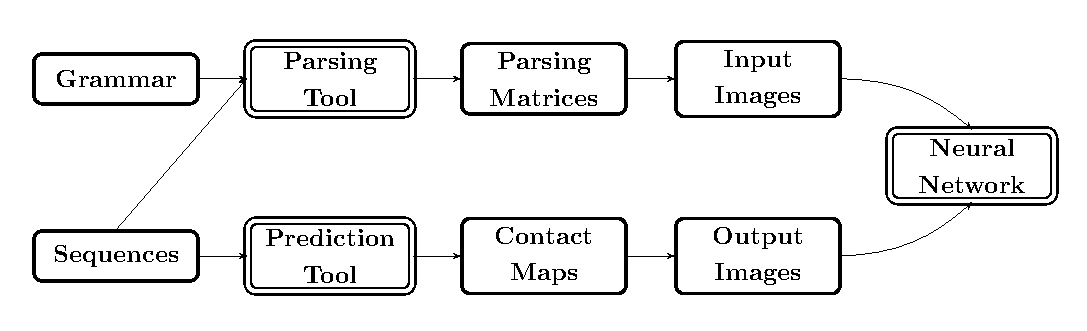
\includegraphics[width=16cm]{pics/schema.pdf}
\caption{Схема решения для предсказания вторичной структуры РНК}
\label{schema}
\end{center}
\end{figure} 

\subsection{Нейронные сети}
Для создания и обучения нейронных сетей в данной работе были использованы библиотека Keras~\cite{chollet2015keras} и фреймворк Tensorflow~\cite{tensorflow2015-whitepaper}.

Рассмотрим общую модель генеративной нейронной сети, разработанной в рамках данной работы. Входными и выходными данными являются изображения, и в рамках поставленной задачи необходимо найти достаточно сложные закономерности между элементами данных, находящимися на большом расстоянии друг от друга, поэтому была использована глубокая сверточная нейронная сеть. Для оптимизации процесса обучения и повышения скорости сходимости была использована технология остаточных нейронных сетей (residual networks), которая основана на добавлении дополнительных связей между отделенными друг от друга слоями. Типичный блок (residual unit) сети, используемой в описанных ниже экспериментах представлен на рис.~\ref{unit}.

\begin{figure}[h]
\begin{center}
\centering
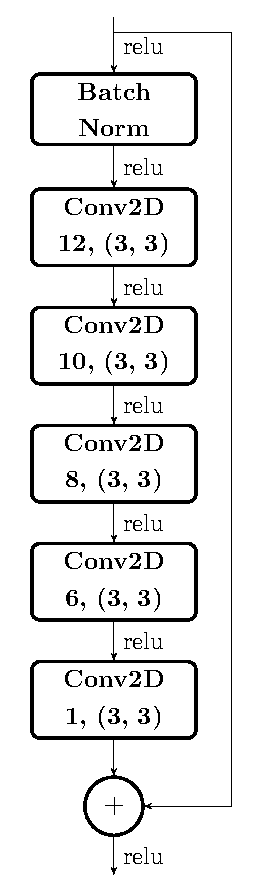
\includegraphics[width=2.5cm]{pics/res_unit.pdf}
\caption{Residual unit}
\label{unit}
\end{center}
\end{figure} 

Для вычисления ошибки нейронной сети при обучении была использована просуммированная попиксельная разница эталона и предсказанного изображения с некоторым коэффициентом $k > 1$ при белых пикселях в эталонных изображениях. Наличие коэффициента было обусловлено тем, что белые пиксели, обозначающие контакт в матрице, составляют малую часть изображения, следовательно, взятие чистой попиксельной разницы не было бы чувствительно к небольшим ошибкам в белых пикселях, которые, тем не менее, привели бы к существенным ошибкам в плане предсказания вторичной структуры. 

Формально, если $p_{e}$ --- нормированное значение пикселя эталонного изображения, а $p_{p}$ --- нормированное значение пикселя предсказанного изображения, то 
\[WeightedLoss = \frac{|\sum \omega - \sum \omega \ast \delta |}{\sum \omega},\] 
\[\omega = (k - 1) \ast p_{e} + 1, \delta = 1 - |p_{e} - p_{p}|.\]

\subsubsection{Метрики}
Для тестирования обученных нейронных сетей были выбраны следующие метрики.
\begin{itemize}
    \item Оценка попиксельной разницы между предсказанным и эталонным изображениями. Далее $TW$ (true white), $TB$ (true black), $FW$ (false white) и $FB$ (false black) --- информация о том, сколько раз нейронная сеть приняла верное и сколько раз неверное решение по каждому пикселю каждого изображения выборки.
    \begin{itemize}
        \item $Precision = \frac{TW}{TW + FW}$ (какая доля предсказанных контактов действительно является контактами в эталоне).
        \item $Recall = \frac{TW}{TW + FB}$ (какая доля искомых контактов была найдена).
        \item $FMera = 2 * \frac{Precision * Recall}{Precision + Recall}$ (гармоническое среднее $Precision$ и $Recall$ --- объединяющая метрика).
    \end{itemize}
    \item Оценка корректности полученной вторичной структуры с точки зрения формата dot-bracket (матричное представление вторичной структуры однозначно представимо в виде скобочной последовательности).
     \begin{itemize}
        \item $LevDist$ (расстояние Левенштейна --- минимальное количество односимвольных операций, т.е. вставки, удаления или замены, необходимых для превращения предсказанной скобочной последовательностей в эталонную).
    \end{itemize}   
\end{itemize}

\section{Эксперименты}
\subsection{Предсказание вторичных структур тРНК фиксированной длины}
Первой задачей для экспериментального исследования применимости предложенной архитектуры к реальным биологическим данным было предсказание вторичной структуры тРНК фиксированный длины $l$. 

Задачи, связанные с подготовкой данных, были выполнены в рамках курсовой работы Кутленкова Дмитрия Александрович на кафедре системного программирования. Цепочки тРНК были взяты из базы данных RNAcentral~\cite{rnacentral}, а эталонные структуры были получены при помощи инструмента CentroidFold~\cite{sato2009centroidfold}. В данном инструменте не реализована возможность предсказания псевдоузлов, однако простота и удобство использования позволили выбрать его в качестве источника данных для первых экспериментов. В качестве $l$ была выбрана длина цепочки в 90 нуклеотидов как средняя для тРНК и самая часто встречающаяся в выбранной базе данных. Для эксперимента было взято 56689 цепочек, поделенных в соотношении train:valid:test = 70\%:10\%:20\%. Реализованная нейронная сеть состояла из десяти residual блоков, конструкция которых описана в разделе 3.4.

Обученная нейронная сеть была протестирована в соответствии с метриками, заданными в разделе 3.4.1 данной работы. Метрики $Precision$, $Recall$ и $FMera$ были вычислены для каждого изображения, а затем взяты средние значения по выборке. Результаты по тестовой выборке представлены в таблице~\ref{table1}.

\begin{table}[h]
\begin{tabular}{|P{2.2cm}|P{2.2cm}|P{2.2cm}|P{2.2cm}|P{2.2cm}|P{2.2cm}|}
\hline
Length & Samples & Alignment & Precision & Recall & F1 score \\ \hline \hline
\multirow{2}{*}{90} & \multirow{2}{*}{26511} & $\times$ & 67\% & 75\% & 68\% \\ \cline{3-6} 
 &  & \checkmark & 80\% & 66\% & 70\% \\ \hline \hline
\multirow{2}{*}{88-90} & \multirow{2}{*}{77976} & $\times$ & 66\% & 78\% & 69\% \\ \cline{3-6} 
 &  & \checkmark & 81\% & 62\% & 68\% \\ \hline \hline
\multirow{2}{*}{50-90} & \multirow{2}{*}{141835} & $\times$ & 60\% & 72\% & 63\% \\ \cline{3-6} 
 &  & \checkmark & 71\% & 61\% & 63\% \\ \hline
\end{tabular}
\caption{Результаты тестирования моделей для данных без псевдоузлов}
\label{table1}
\end{table}

\subsubsection{Выравнивание}
Как можно увидеть по таблице~\ref{table1}, была получена достаточно высокая точность предсказания контактов между нуклеотидами. Однако, большая доля предсказанных изображений не преобразуется в валидную вторичную структуру в формате dot-bracket (строка "error" в таблице~\ref{table1}). Так происходит в том случае, когда в сгенерированном изображении у одного нуклеотида сразу несколько пар (т.е. в одной строке более одного белого пикселя), тем не менее, во вторичной структуре без псевдоузлов такое невозможно. Это означает, что, несмотря на то, что нейронная сеть успешно находит значительную часть контактов во вторичной структуре, она при этом допускает ошибки с точки зрения биологической корректности результата. 

Для решения данной проблемы был использован алгоритм локального выравнивания последовательностей, разработанный и реализованный в рамках курсовой работы Кутленкова Дмитрия Александровича на кафедре системного программирования. Данный алгоритм на основании сгенерированного нейронной сетью изображения получает вторичную структуру, удовлетворяющую биологическим законам. Однако непосредственное применение алгоритма к результатам работы нейронной сети привело к падению точности, поэтому было принято решение сделать его адаптивным, т.е. встроить выравниватель как финальный слой нейронной сети и дообучить оригинальную модель с выравнивающей надстройкой. При дообучении была использована другая функция loss: линейная комбинация $WeightedLoss$ и $1 - FMera$. Результаты тестирования комбинированной нейронной сети по стандартным метрикам представлены в таблице~\ref{table2}. 

\begin{table}[h]
\begin{tabular}{|P{1.5cm}|P{1.5cm}|P{1.5cm}|P{1.5cm}|P{1.5cm}|P{1.5cm}|}
\hline
Length & Samples & Alignment & Precision & Recall & F1 score \\ \hline \hline
50-90 & 266 & $\times$ & 74\% & 73\% & 71\% \\ \hline
\end{tabular}
\caption{Средние значения метрик на тестовой выборке}
\label{table2}
\end{table}

Видно, что выравнивание позволило существенно сократить процент ошибок, повысив при этом и процент точно предсказанных вторичных структур. Таким образом, изучение данной техники и более тонкая настройка параметров модели требует дальнейших исследований.

\subsection{Предсказание вторичных структур тРНК произвольной длины}
Эксперимент с цепочками фиксированной длины показал достаточно высокую точность результата, но реальные последовательности тРНК имеют очень разную длину, поэтому было необходимо также реализовать модель, предсказывающую вторичную структуру для произвольной длины последовательности. Для этого были отобраны 145054 цепочки длин от 50 до 90 символов из той же самой базы RNAcentral и аналогичным образом получены их вторичные структуры с помощью инструмента CentroidFold. Данные были поделены на обучающую, валидационную и тестовую выборки в том же соотношении 70\%:10\5:20\% и была использована такая же архитектура нейронной сети, как и в разделе 4.1, но в данном эксперименте изображения при обучении распределялись на батчи так, чтобы в каждом батче присутствовали изображения только одного размера.
Результаты оценки результатов по метрикам $Precision$, $Recall$, $FMera$ и $LevDist$ представлены в таблице~\ref{table3}.

\begin{table}[h]
\centering
\begin{tabular}{|p{2cm}|p{2cm}||p{2cm}|p{2cm}|}
\hline
\multirow{2}{*}{Precision} & \multirow{2}{*}{56\%} & LevDist & Samples \\ \cline{3-4} 
 &  & 0 & 1\% \\ \hline
\multirow{2}{*}{Recall} & \multirow{2}{*}{75\%} & 1-5 & 6\% \\ \cline{3-4} 
 &  & 6-10 & 11\% \\ \hline
\multirow{2}{*}{FMera} & \multirow{2}{*}{62\%} & \textgreater{}10 & 26\% \\ \cline{3-4} 
 &  & error &56\% \\ \hline
\end{tabular}
\caption{Результаты тестирования модели для длин 50-90}
\label{table3}
\end{table}

Полученные результаты говорят о том, что теоретически предсказание вторичной структуры для цепочек разных длин в рамках предложенного подхода возможно, однако необходимы дальнейшие эксперименты.

\subsubsection{Предсказание псевдоузлов}
Одной из задач, поставленных в данной работе, было изучение возможности предсказания вторичной структуры для цепочек, содержащих псевдоузлы. Псевдоузлы невыразимы средствами контекстно- \linebreak свободных грамматик, поэтому было необходимо проверить, насколько точно можно достроить их по матрице разбора с помощью нейронной сети.

В данном эксперименте было взято 275 цепочек со вторичными структурами из базы Pseudobase~\cite{pseudobase}, train:valid:test = 70\%:10\%:20. Цепочки имели различные длины, поэтому были использованы веса модели из раздела 4.2 с последующем дообучением. Тестирование проводилось по метрикам $Precision$, $Recall$ и $FMera$ и результаты продемонстрированы в таблице~\ref{table4}

\begin{table}[h]
\begin{tabular}{|l|l|}
\hline
\multirow{2}{*}{Precision} & \multirow{2}{*}{78\%} \\
 &  \\ \hline
\multirow{2}{*}{Recall} & \multirow{2}{*}{75\%} \\
 &  \\ \hline
\multirow{2}{*}{FMera} & \multirow{2}{*}{75\%} \\
 &  \\ \hline
\end{tabular}
\caption{Результаты тестирования модели для данных с псевдоузлами}
\label{table4}
\end{table}

Тестирование по скобочным последовательностям на данный момент не проводилось, поэтому судить о точности предсказания именно псевдоузлов пока рано, но, тем не менее, можно увидеть, что данная модель показала лучший результат, чем та, на которой она была основана, что позволяет полагать, что у задачи предсказания псевдоузлов есть потенциал.

% У заключения нет номера главы
\section*{Заключение}
В данной работе было проведено исследование возможности применения подхода, основанного на комбинировании формальных грамматик и нейронных сетей, к задаче предсказания вторичных структур РНК. Были получены следующие результаты.
\begin{itemize}
    \item Разработана архитектура решения.
    \item Проведены экспериментальные исследования применительно к задачам предсказания вторичных структур транспортных РНК.
\end{itemize}

Направлениями дальнейших исследований являются следующие задачи.
\begin{itemize}
    \item Более тщательная разработка модели, применяющей адаптивное выравнивание.
    \item Повышение точности нейронной сети, обучающейся на изображениях произвольного размера.
    \item Реализация системы тестирования результатов работы нейронных сетей на данных с псевдоузлами.
    \item Поиск новых средств, а также более тонкая настройка параметров всех моделей для улучшения результатов.
\end{itemize}

\setmonofont[Mapping=tex-text]{CMU Typewriter Text}
\bibliographystyle{ugost2008ls}
\renewcommand\refname{Список литературы}
\bibliography{diploma.bib}
\end{document}